\section{Introduction}
% Delete the text and write your Introduction here:
%------------------------------------

In recent years, the fields of Reinforcement Learning (RL) and Genetic Algorithms (GA) have garnered significant attention for their ability to tackle complex optimization problems. Both techniques, despite their distinct methodologies, are really good at solving reinforcement learning problems. That is due to their main function  \cite{taylor2006comparing}. 

%n Machine learning, several methods can be used to solve the same problem. For example, trying to find the local minima using evolutionary algorithms or supervised learning in the form of backpropagation. Both come with advantages and disadvantages depending on if we are after precision or just want to find the local minima fast, but also depending on the nature of our problem.

More specifically interesting is the comparison of the performance of Genetic Algorithms (GA) and Reinforcement Learning (RL) techniques in the context of a game environment. On one hand, in reinforcement learning the agent engages a dynamic and evolving environment by taking actions that affect it to accomplish a specific goal (solve an RL problem). On the other hand, we have evolutionary algorithms that employ evolutionary principles for automated and concurrent problem-solving drawing inspiration from populations of evolving organisms. Despite their apparent dissimilarities, RL and GA both tackle the same fundamental issue: optimizing a function. This entails maximizing an agent's reward in RL and the fitness function in evolutionary algorithms, respectively, particularly in environments where the parameters may be unknown \cite{drugan2019reinforcement}.  

 One prevalent use of genetic algorithms often lies in optimizing multiparameter functions. Numerous problems can be framed as a quest for the optimal value, where this value represents a complex function of various input parameters. \cite{forrest1996genetic}. More specifically \textit{temporal difference methods} , a division of RL,  learns a value function, which estimates the anticipated long-term reward associated with taking a specific action in a given state. Alternatively, genetic algorithms (GAs) offer another avenue for addressing RL problems by exploring the policy space to identify the one yielding maximum reward \cite{taylor2006comparing}. 

This paper compares Reinforcement learning and Genetic Algorthms by having them balance a cartpole in 500 moves. More specifically it is a problem in nonlinear dynamics where an inverted pendulum is balancing in a cart. The aim or final goal of both RL and GA are to keep it the system balanced until they run out of moves. A graphic representation can of the environment can be seen in Figure \ref{figPOLE}. The environment will be described in more detail under the environment part.  
\begin{figure}[H]
    \centering
    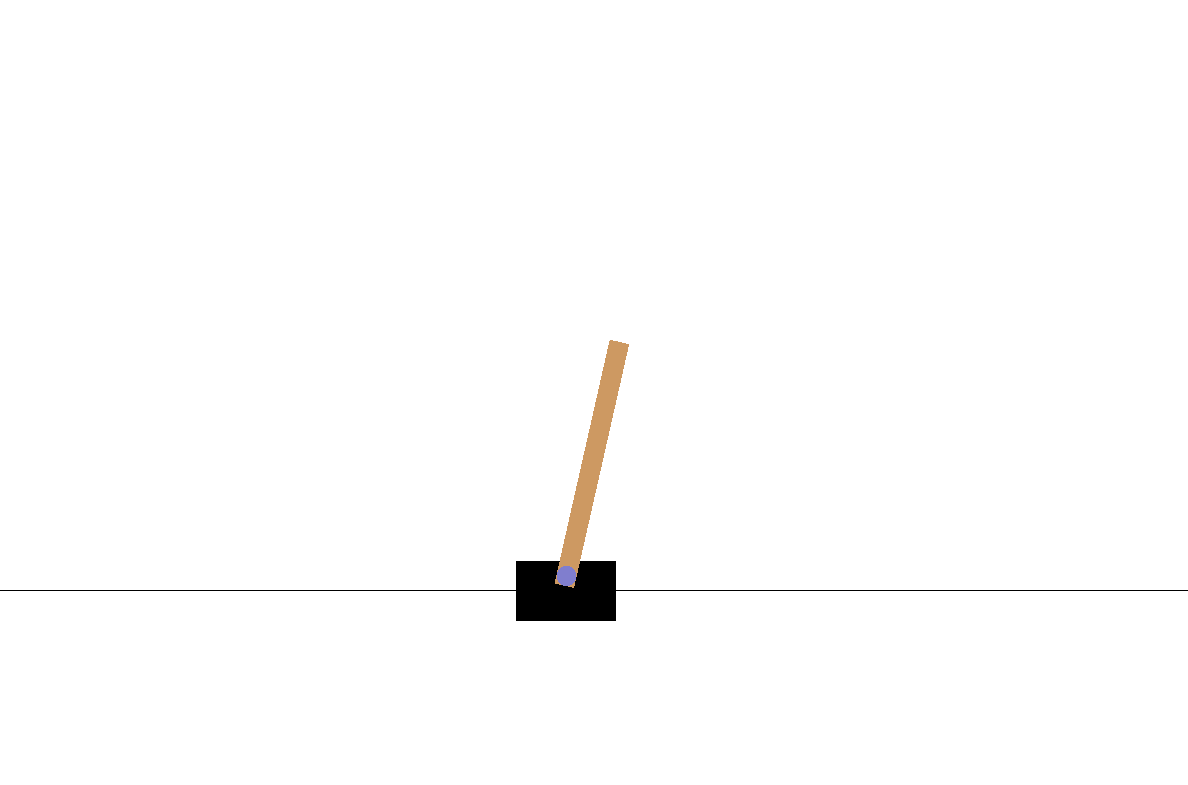
\includegraphics [scale = 0.18]{Images/cartpole.png}
    \caption{The cartpole in 2D graphics}
    \label{figPOLE}
\end{figure}


